\subsection{Learning rate}

A continuación incluímos los resultados de los experimentos en donde comparamos la forma en que el
QLearn player aprende a jugar contra distintos tipos de jugadores, para una cantidad de juegos entre
1 y 100.000.

Realizamos 3 corridas diferentes, en donde variamos el rol del QLearn player en el juego: Jugador
que realiza el primer movimiento, que mueve segundo o alternando los turnos de inicio.

Los parámetros del QLearn Player fueron fijados con los siguientes valores:
$\epsilon$ = 0.2, $\alpha$ = 0.3, $\gamma$ = 0.9

\begin{figure}
	\centerline{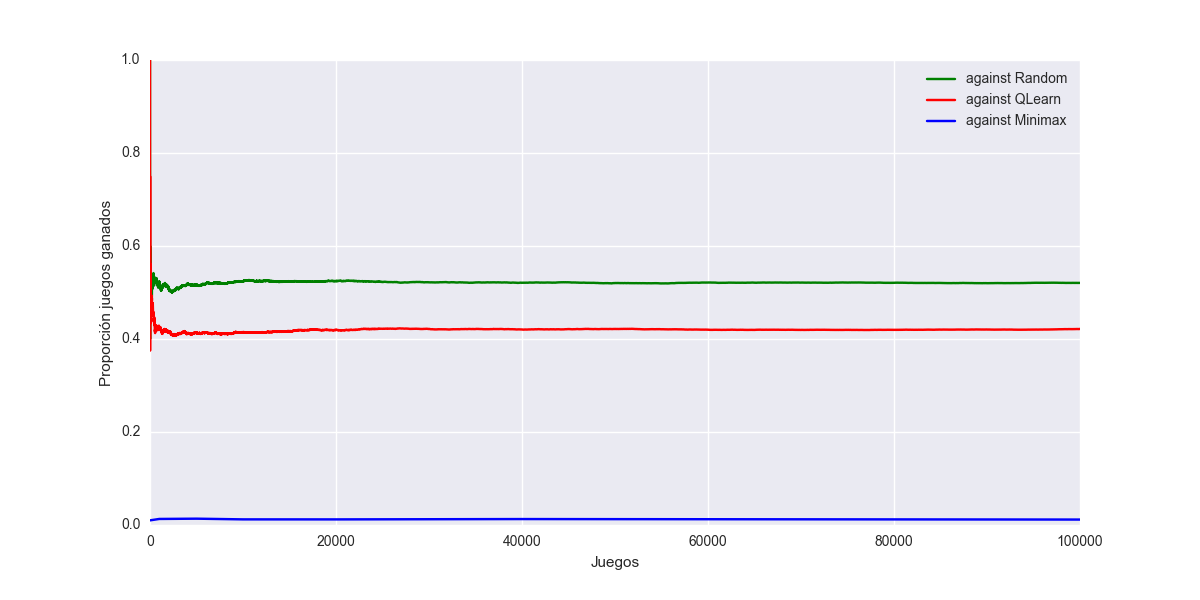
\includegraphics[width=1.3\textwidth]{figures/learning_rate_as_second_player.png}}
	\caption{Porcentaje de victorias como jugador que mueve segundo}
\end{figure}

\begin{figure}
	\centerline{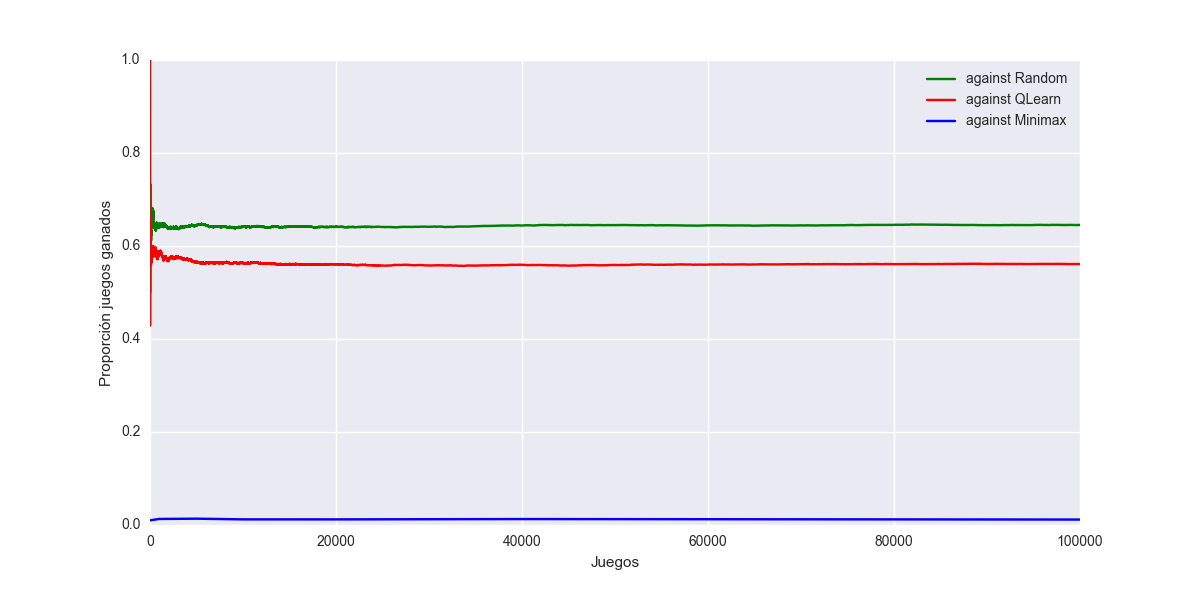
\includegraphics[width=1.3\textwidth]{figures/learning_rate_as_first_player.png}}
	\caption{Porcentaje de victorias como jugador que mueve primero}
\end{figure}

\begin{figure}
	\centerline{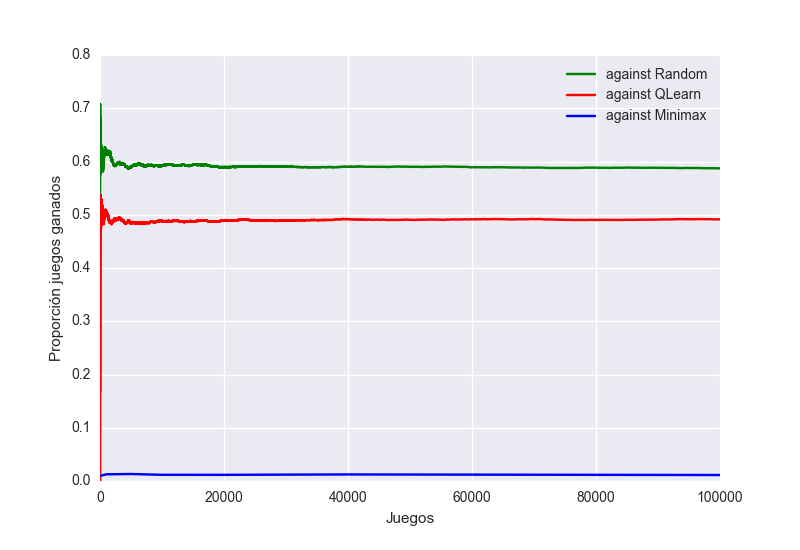
\includegraphics[width=1.3\textwidth]{figures/learning_rate_rotating_turns.png}}
	\caption{Porcentaje de victorias alternando los turnos de inicio}
\end{figure}

En los 3 casos observamos malos resultados. El porcentaje de victorias permanece constante para esa cantidad
de juegos, lo que da un indicio de que el algoritmo no obtiene mejoras inmediatas en su aprendizaje según
el tipo de jugador ni dependiendo de si empieza primero o segundo (aunque obtiene más victorias cuando
mueve primero).
